%----------------------------------------------------------------------------------------
%	PACKAGES AND DOCUMENT CONFIGURATIONS
%----------------------------------------------------------------------------------------
\documentclass[a4paper,11pt]{article}
\usepackage{amsmath} % Required for some math elements
\usepackage{hyperref} 
\usepackage{xcolor}
\usepackage{lipsum} 
\usepackage{cite}
\usepackage{graphicx} % Required for the inclusion of images
\usepackage{algorithmic}
\usepackage{array}
\usepackage{bookmark}
\usepackage{listings}
\usepackage{mcode}
\usepackage{amssymb}
\usepackage{enumitem}
\usepackage[margin=20mm,]{geometry}
\usepackage[caption=false, font=footnotesize]{subfig}

\newlist{steps}{enumerate}{1}
\setlist[steps, 1]{label = Step \arabic*:}

\hypersetup{ %color attributes of citation, link, etc.
    colorlinks=true,
    linkcolor=blue,
    filecolor=gray,      
    urlcolor=blue,
    citecolor=blue,
}

\newcommand{\matlab}{\textsc{Matlab }} %very important and totally necessary addition

\newcommand\Item[1][]{%
  \ifx\relax#1\relax  \item \else \item[#1] \fi
  \abovedisplayskip=0pt\abovedisplayshortskip=0pt~\vspace*{-\baselineskip}}
  %----------------------------------------------------------------------------------------
%	DOCUMENT INFORMATION
%----------------------------------------------------------------------------------------
 
\title{ECEN315 LABORATORY REPORT ONE}
\author{Daniel Eisen : 300447549}
\date{\today}

\begin{document}
\maketitle
\section{Introduction}
This project has the goal of creating a system for controlling a pendulum arm driven by a propeller. This necessitates the modelling of system, breaking it into sub-blocks/sub-systems and evaluating these models. The work outlined in this report covers the modelling of the Motor/Propeller and the Pendulum subsystems, the measured values for the physical system constants, deriving those that couldn't be directly measured, and how these systems combine in relation to the full open loop model of the system.

\section{Background}
\subsubsection*{Control}
Control theory deals with the control of dynamic systems with the objective to develop a model for controlling such systems by driving this system to result in an optimum output without delay or overshoot and stability.

Delay refers to the speed of the systems response to an input. \\
Overshoot is the degree of which the response becomes greater than the desired value.\\
Stability is defined as the final value of the system being bounded and finite.

Extensive use of the block diagram is use to model these systems. In it is the transfer function, this is the model of relation between the input and output based on the differential equations describing the system, this is usually represented in the S domain.

\subsubsection*{DC Motors}
A DC motor consists of both an electrical and a mechanical subsystem. It converts electrical energy into mechanical energy in its motor application. It can be broken down into sub-blocks representing the the \textit{Electrical Subsystem} that then drives the \textit{Mechanical Subsystem} via \textit{Torque Coupling} to produce rotational output (of the shaft). This also produces a back emf, in the form of negative feedback into the system.   
\subsubsection*{Pendulum}
The pendulum modelled, is what is known as a Compound Pendulum \cite{pen}. Meaning its motion is subject not only to the effects of gravity around its centre of mass (as the arm has mass), but also its inertia in relation to its angular acceleration and the damping (via pivot friction) to its angular velocity. 

\newpage
\section{Methodology and Results}
In this section you will explain how to solve the problem, that is, how you performed the project. At this early stage you need to be both clear about what you did and why you did it. You will also explain how you evaluated your solution once you have built it. The method of evaluation will be specific to the tasks. 
\subsection{DC Motor and Propeller}
\begin{figure}[h]
        \centering
        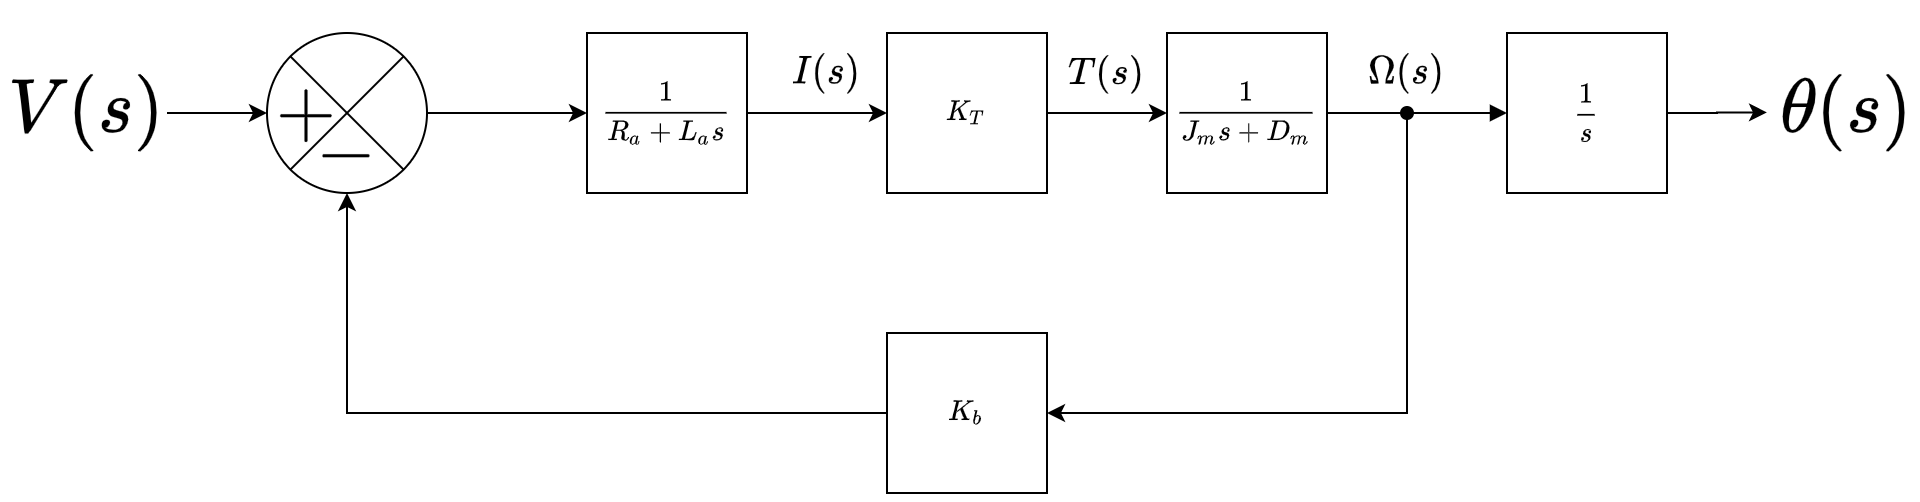
\includegraphics[width=0.75\textwidth]{inc/motor_diagram.png}
        \caption{Block Diagram of DC Motor+Propeller System}
        \label{}
\end{figure}

As outlined in Gideon Gouws DC motor documentation \cite{dcmotors}, the DC+propeller's rotational velocity ($\Omega(s)$) system can be modelled by the above block diagram in figure 1. This was then combined and reduced to form a transfer function (representing the sub-system) of inputted voltage to outputted angular velocity.

\begin{align*}
        \frac{\Omega(s)}{V(s)} &= \frac{\frac{K_t}{(R_a+L_{a}s)(D_m+J_{m}s)}}{1+\frac{K_tK_b}{(R_a+L_{a}s)(D_m+J_{m}s)}} \\
                               &= \frac{K_t}{(R_a + L_{a}s)(D_m+J_{m}s) + K_tK_b} \\
                               &= \frac{K_t}{L_aJ_{m}s^{2} + (R_{a}J_{m} + L_aD_{m})s + R_{a}D_{m} + K_tK_b } \\
                               &= \frac{\frac{K_t}{L_aJ_m}}{s^2 + \frac{R_{a}J_{m} + L_{a}D_{m}}{L_{a}J_{a}}s + \frac{R_aD_m + K_tK_b}{L_aJ_m}}
\end{align*}

The values of the these physical constants, were measured (multiple times) from the physical system in a previous year then averaged to get the final, utilised values. Using the constants and the derived transfer function, the sub-system was modelled in \matlab. A multi-step input analysis at V = [1, 2, 3, 4, 5, 6], the results of which are shown in figure 2. This shows the settling time of the system as well as the respective steady state values for each input. The script also computed the steady state gain, $SSG = 80.631551 \frac{rad}{Vs}$ and the Time constant, $\tau = \sqrt{\tau_1 \tau_2} = \sqrt{\frac{1}{\omega_1 \zeta_1} \frac{1}{\omega_2 \zeta_2}} = 0.196093$

\begin{figure}[h]
        \centering
        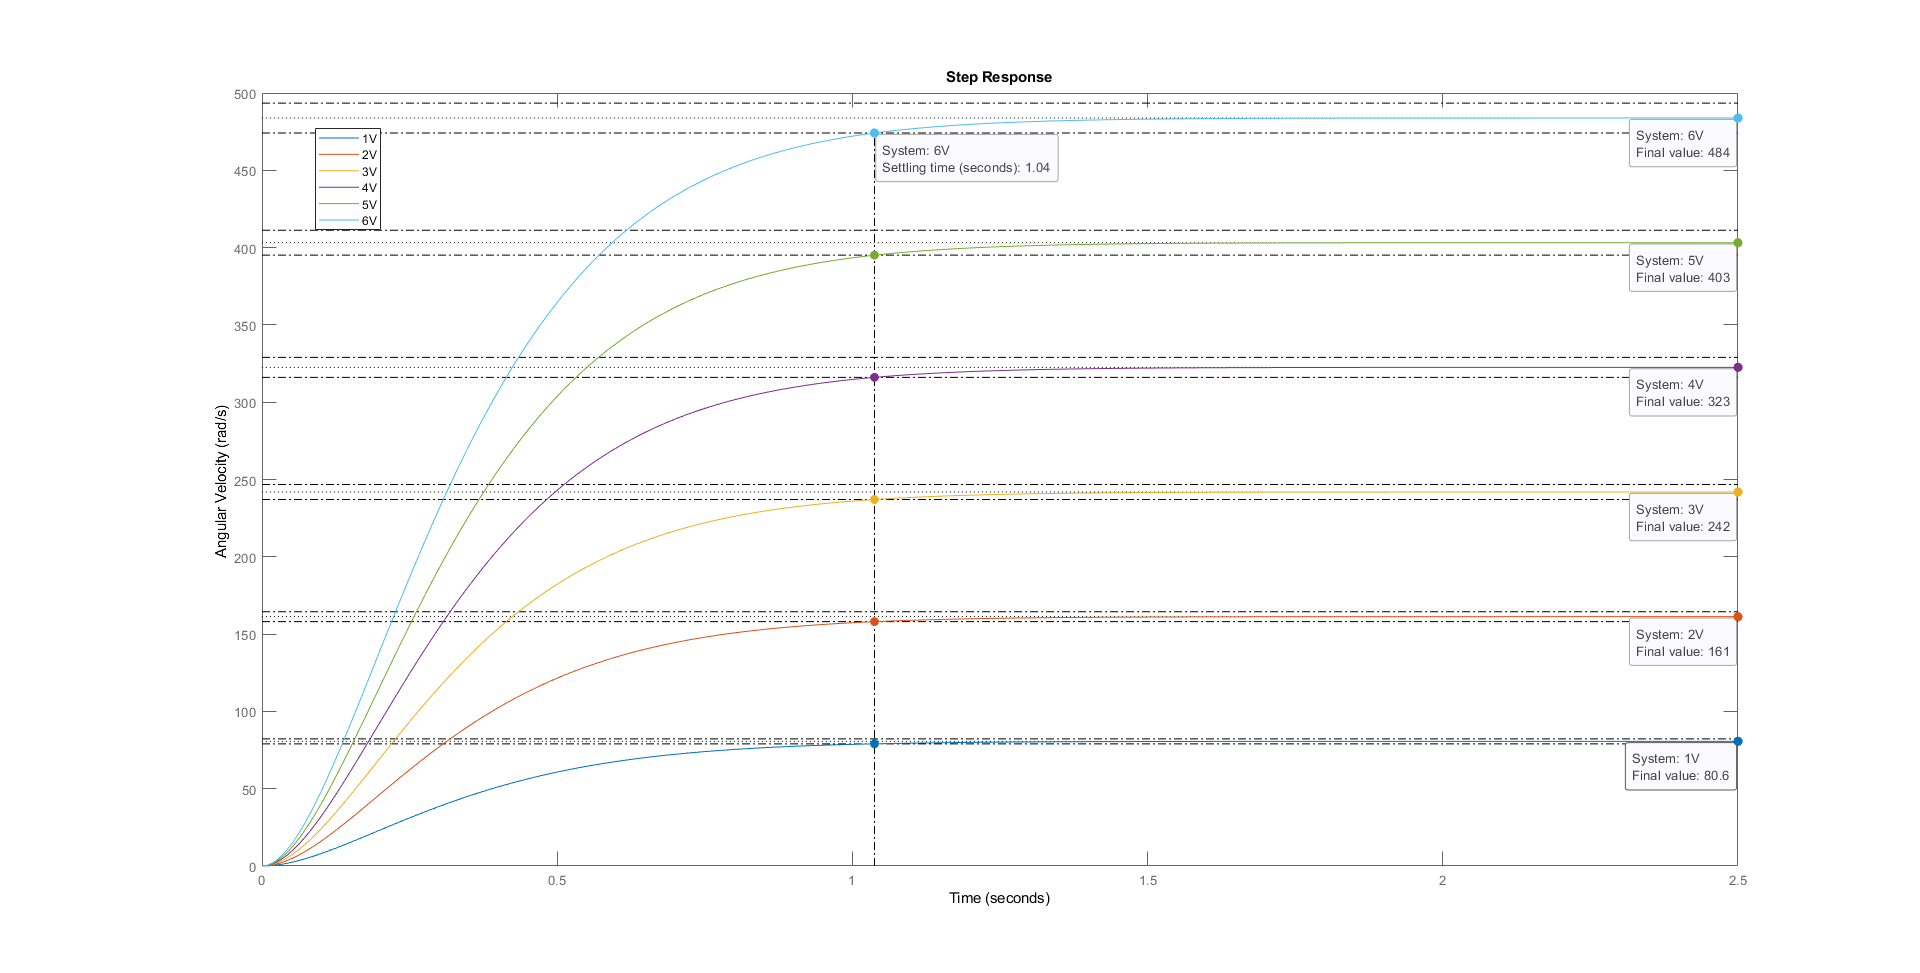
\includegraphics[width=\textwidth]{inc/motor_steps.png}
        \caption{Step response}
        \label{}
\end{figure}

\newpage
\subsection{Pendulum}
The pendulum sub-block represents the conversion of input torque (via the thrust provided from the propeller)
For the driven pendulum, the torque applied to the pendulum must balance with the existing torques, ie from gravity, damping and the arms moment of inertia. Before the DE is derived, I needed to approximate the torque applied via gravity:
$$\tau_{gravity} = mgd{\cdot}sin(\theta) = mgd{\cdot}\theta$$
This approximation works for small angles, but quickly diverges in accuracy for $\theta \ge \pi/8 \rightarrow \pi/4$ \\

\begin{center}
        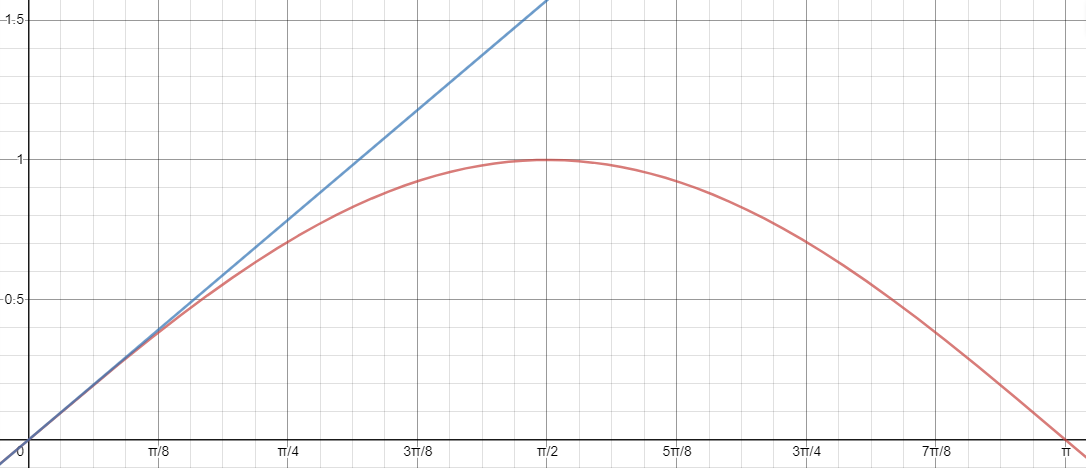
\includegraphics[width=0.45\textwidth]{inc/sintheta.png}
\end{center}
\subsubsection{Differential Equation and Transfer Function}
The input torque is the thrust force generated by the propeller, F, along the length of the arm, r. This balanced by the 3 components of torque on the arm. Its moment of inertia ($J_p$) by the rotational acceleration, the linear damping $c$ by the rotational velocity and the force of gravity at the centre of mass ($mgd$) by the rotation. This forms the below differential equation and following transfer function.
\begin{align*}
\tau(t) &= J_{p}\frac{d^{2}\theta}{dt^{2}} + c\frac{d\theta}{dt} + mgd\theta \\
T(s) &= J_{p}s^{2}\Theta(s) + cs\Theta(s) + mgd\Theta(s) \\
\frac{\Theta(s)}{T(s)} &= \frac{1}{J_{p}s^{2} + cs + mgd} \\
&=  \frac{\frac{1}{J_{p}}}{s^{2} + \frac{c}{J_{p}}s + \frac{mgd}{J_{p}}}
\end{align*}


\subsubsection{Fitting Undriven Pendulum Curve}
All constants but $c$ and $J_P$ could be easily measured. So data measured from the disturbance of a the undriven pendulum and fit the decay exponential, $Ae^{-Bt}$ to get A and B.
\begin{figure}[h]
        \centering
        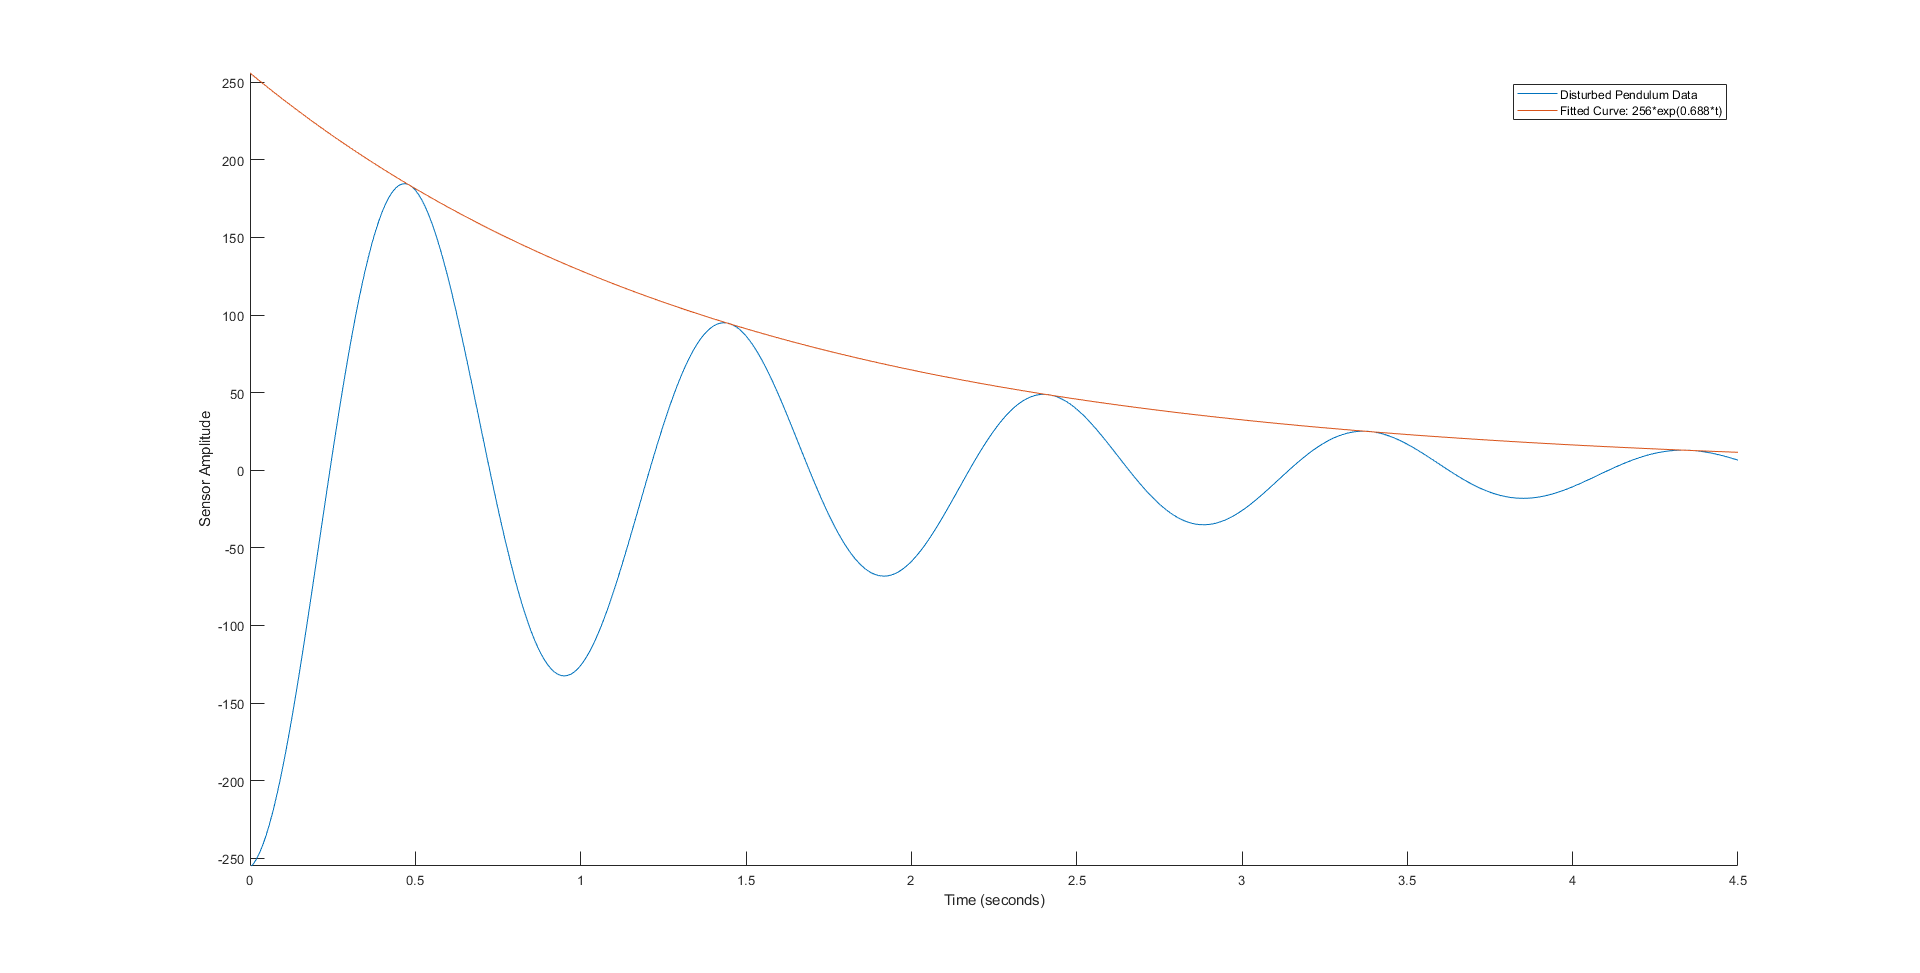
\includegraphics[width=0.7\textwidth]{inc/fittedcurve.png}
        \caption{}
        \label{}
\end{figure}

Figure 3 show the curve envelope fit to the oscillation peaks, Setting A to max sensor output then tuning B. This gave values of A = 256, and B = 0.688.
By inspection, the period T of the signal can be read. Using it to get $\omega = \frac{2\pi}{1.43-0.47}$

\subsubsection{Calculating Damping and Inertia}
Given that $\omega = \sqrt{\frac{mgd}{J_p}-B^2}$, the moment of inertia and damping coefficient can be calculated:
$$J_p = \frac{mgd}{\omega^2 + B^2 = 0.0053}\;\;\;\;\;\;\;\;c = 2J_{p}B = 0.0073$$

So now with all the constants know, the step response of this system is plotted below with the peak response and settling time marked. Though this is for a step input of 0.1, to better represent the actual values that it would be driven at.
\begin{figure}[h]
        \centering
        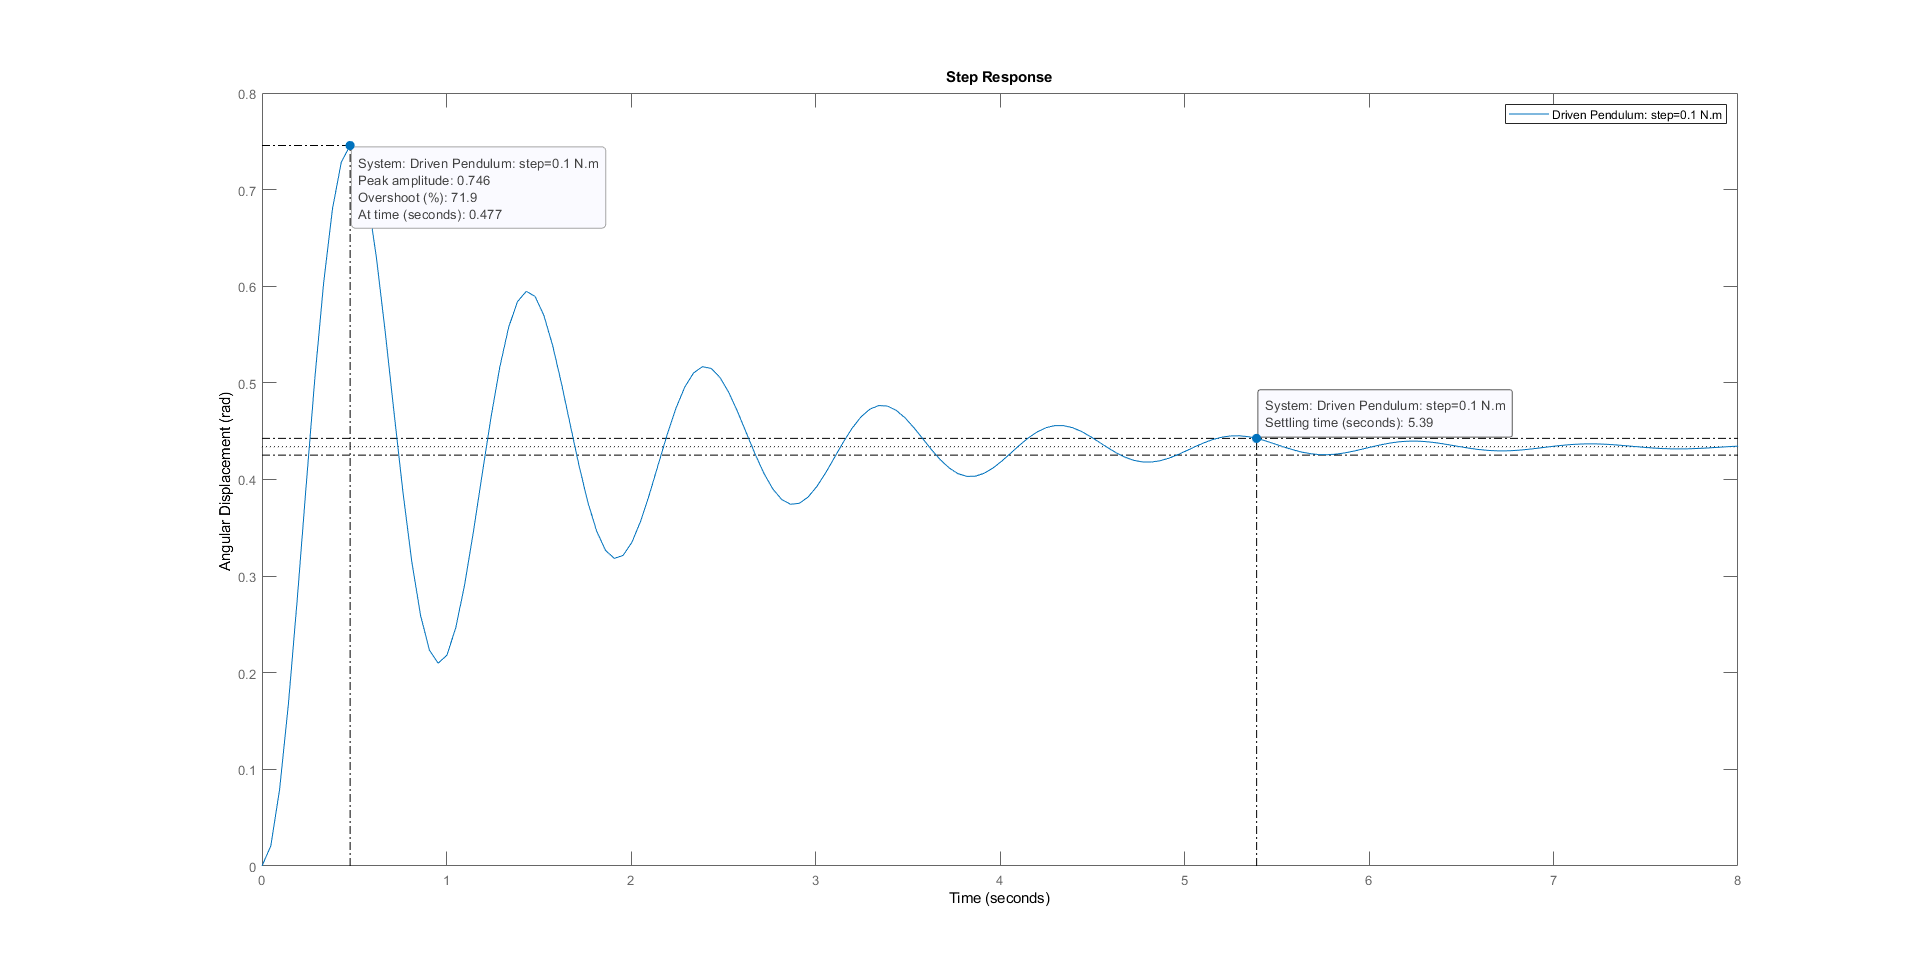
\includegraphics[width=0.75\textwidth]{inc/pendulum.png}
        \caption{}
        \label{}
\end{figure}

\newpage
\subsection*{Full Open Loop TF}
\begin{figure}[h]
        \centering
        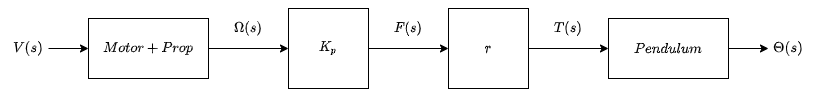
\includegraphics[width=0.75\textwidth]{inc/openloop_diagram.png}
        \caption{Block Diagram of DC Motor+Propeller System}
        \label{}
\end{figure}

As shown in figure 5, the combined system needs to first transform rotational velocity into thrust (force), the block to do so we found via a linear approximation of the measured response $\rightarrow\:K_p$, which is applied over the distance r to provide an input torque to the pendulum. Using the previously derived transfer functions the full system block is shown below.

\begin{align*}
        \frac{\Theta(s)}{V(s)} &= \frac{\frac{K_t}{L_aJ_m}}{s^2 + \frac{R_{a}J_{m} + L_{a}D_{m}}{L_{a}J_{m}}s + \frac{R_aD_m + K_tK_b}{L_aJ_m}} \cdot K_{p} \cdot r \cdot \frac{\frac{1}{J_{p}}}{s^{2} + \frac{c}{J_{p}}s + \frac{mgd}{J_{p}}} \\
        &= \frac{\frac{K_tK_pr}{J_pL_aJ_m}}{(s^2+\frac{c}{J_p}s+\frac{mgd}{J_p})(s^2+\frac{R_aJ_m+L_aD_m}{L_aJ_m}s+\frac{R_aD_m+K_tK_b}{L_aJ_m})}
\end{align*}



\begin{figure}[h]
        \centering
        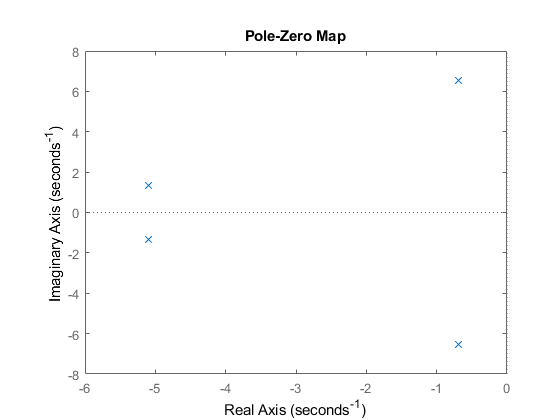
\includegraphics[width=0.39\textwidth]{inc/poles_sys.png}
        \caption{}
        \label{}
\end{figure}

From the poles shown in figure 6, the response can be approximately described as being quite oscillatory due to complex poles and slow acting due to pole not being very negative. And the simulated results are shown in figure 7, With the peak response, settling time and per input steady state values marked.

\begin{figure}[h]
        \centering
        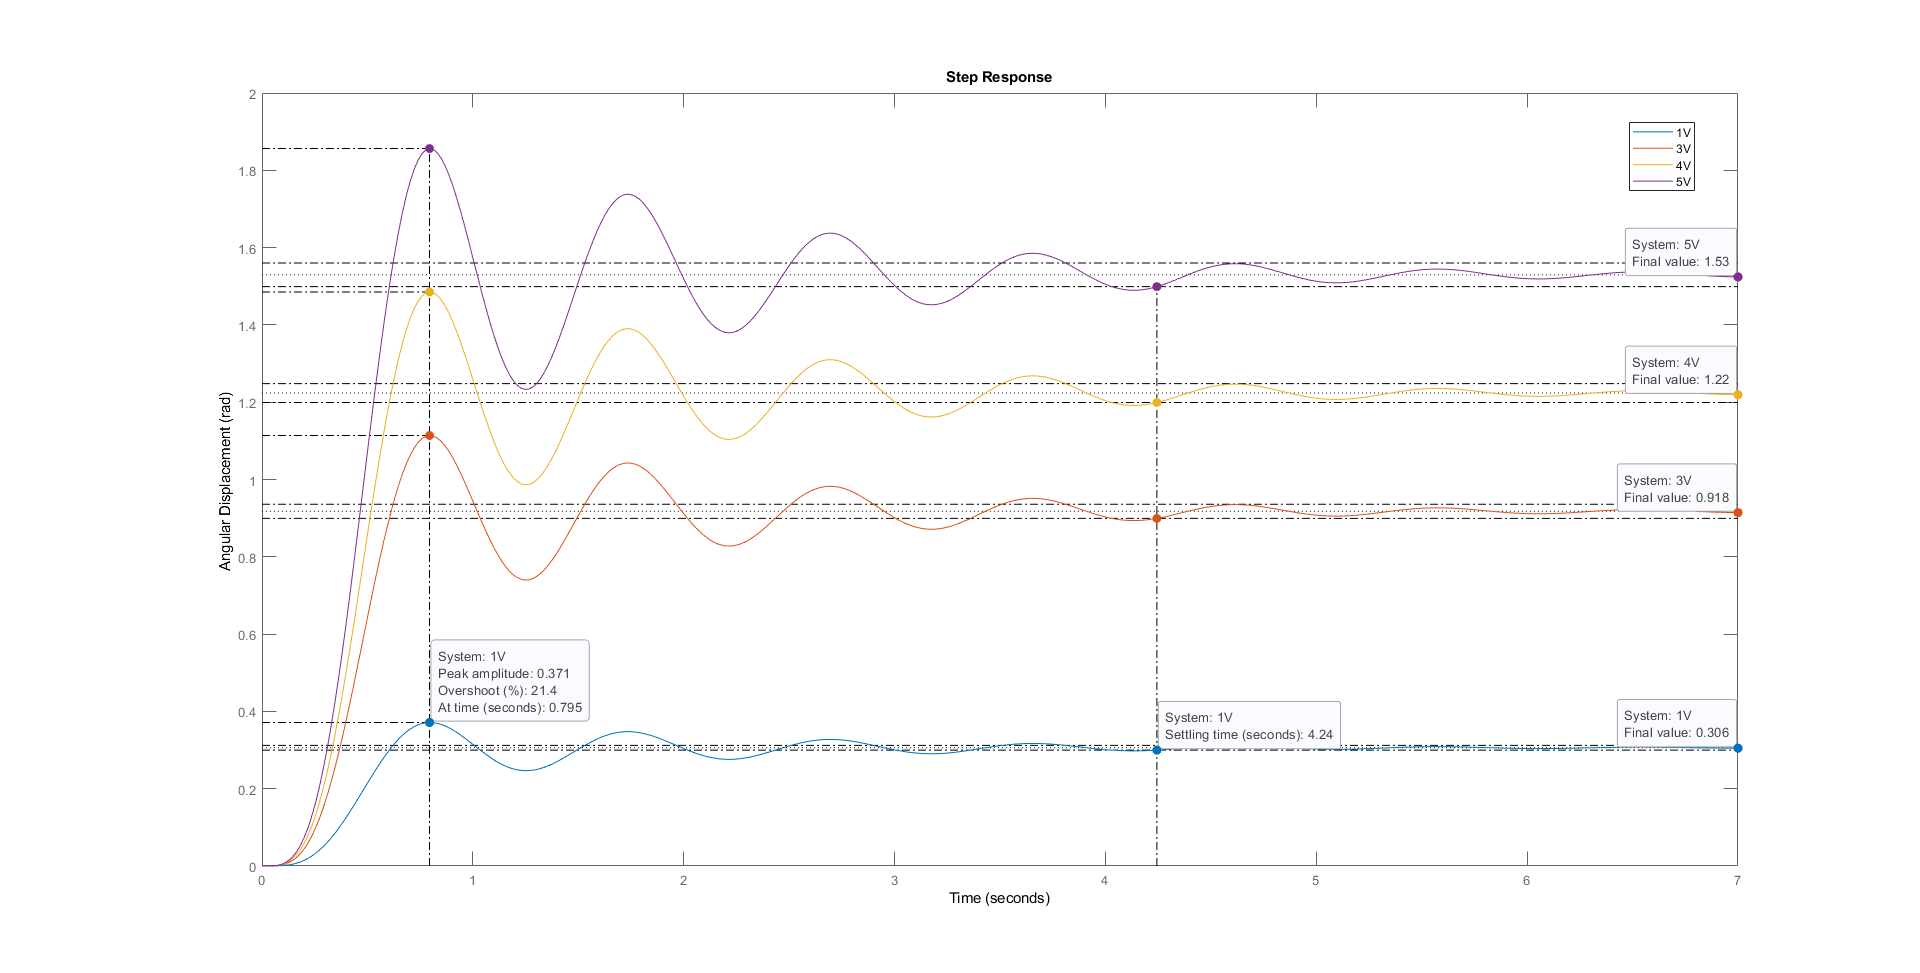
\includegraphics[width=0.7\textwidth]{inc/combined_sys.png}
        \caption{}
        \label{}
\end{figure}

\newpage
\section{Discussion}
The sum results of this report is a model of the open loop system relating the input voltage to a DC motor to the resultant angular displacement of the armature. This will be vital when adding a control system to drive the DC motor. Though it should noted that the model is flawed in some specific places.

Firstly, as previously mentioned the torque applied via gravity on the pendulum was approximated to small angles. This usable from $\theta \le 45^{\circ}$ but will severely alter the actual response for greater angles.

The relation between the angular velocity of the propeller and its produced thrust was also simpler that it should be physically. And thus the real world system will diverge from this model for greater speeds of the propeller.

Also due to the rough derivation of $J_p$ and $c$ of the system, this model could have errors.


These limitation therefore must be taken into account, possibly in the restriction of operating parameter or necessitating great measurement precision.
\section{Conclusions}
In conclusion this is workable open loop representation of the system, suitable for use in designing a control system around, but has limitations and approximations that may introduce divergences from reality.

\bibliography{ref}
\bibliographystyle{IEEEtran}

\newpage

    \section{Full MatLab Code}
    \lstinputlisting{open_loop.m}
    \section{Lab Safety}
    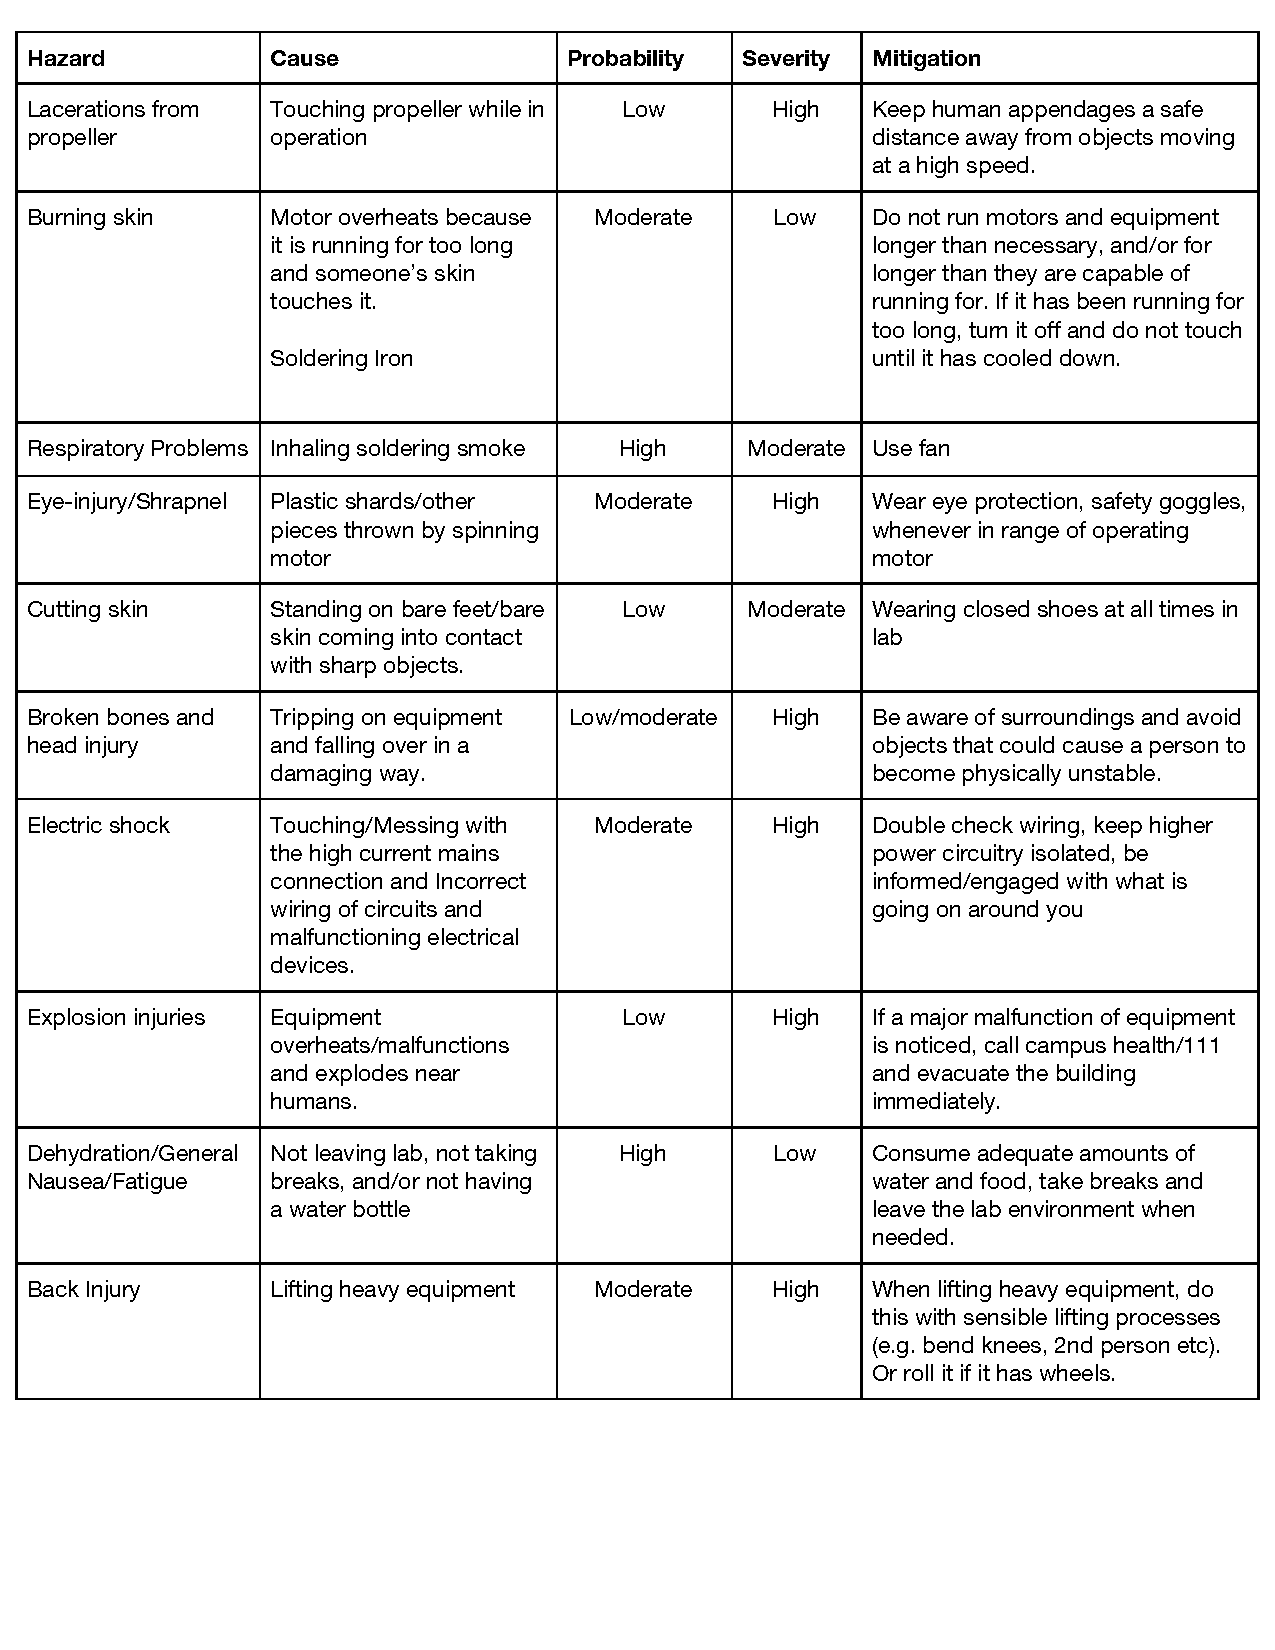
\includegraphics[width=\textwidth]{inc/safety.pdf}
    
\end{document}
